\begin{center}
\Huge
Ekstrema
\end{center}
\section*{Maksima og minima}
\stepcounter{section}

I mange sammenhænge er det en fordel at kunne bestemme \textit{toppunkter/maksima og minima} for en funktion $f$. Hvis $f$ er en differentiabel funktion, så kan vi udnytte differentialregning til at bestemme sådanne punkter. Et punkt, der enten er et maksimum eller et minimum kaldes et \textit{ekstremumspunkt}. 

Vi har følgende sætning:
\begin{setn}[Ekstremumspunkter]
	Lad $f$ være en differentiabel funktion. Hvis et punkt $P(x_0,f(x_0))$ er et ekstremumspunkt for $f$, så gælder der, at 
	\begin{align*}
		f'(x_0) = 0.
	\end{align*}
\end{setn}
Det er dog værd at bemærke, at vi ikke nødvendigvis har den omvendte implikation; hvis $f'(x_0)=0$, så er $(x_0,f(x_0))$ ikke nødvendigvis et ekstremumspunkt. Vi kalder sådanne for \textit{vendetangenter}, og vi vil se eksempler på disse senere. 

\begin{exa}
	Lad $f$ være givet ved
	\begin{align*}
		f(x) = x^3-6x^2+5.
	\end{align*}
	Vi ønsker at bestemme ekstrema for $f$. Vi differentierer derfor først $f$.
	\begin{align*}
		f'(x) = 3x^2-12x = 3x(x-4).
	\end{align*}
	Dette sættes nu lig $0$, og vi får
	\begin{align*}
		3x(x-4) = 0, 
	\end{align*}
	og ved hjælp af nulreglen ved vi, at $x=0$ eller $x = 4$. Vi bestemmer nu de tilhørende $y$-værdier og vi får
	\begin{align*}
		f(0) = 5
	\end{align*}
	og 
	\begin{align*}
		f(4) &= 4^3 - 6\cdot 4^2+5\\
		&= 64-96+5\\
		&= -27.
	\end{align*}
	Vi har derfor en vandret tangent i $P(0,5)$ og $Q(4,-27)$. For at bestemme, om det er et ekstremumspunkt, så tegner vi grafen. Denne kan ses af Fig. \ref{fig:ekstrema}
	\begin{figure}[H]
		\centering
		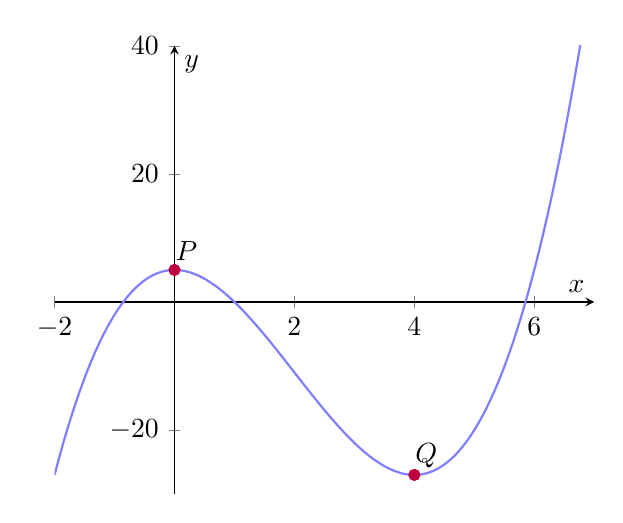
\begin{tikzpicture}
			\begin{axis}[axis lines = middle,
			xmin = -2, xmax = 7,
			ymin = -30, ymax = 40,
			xlabel = $x$, 
			ylabel = $y$]
				\addplot[color = blue!50, samples = 200, domain = -2:7, thick] {x^3-6*x^2+5};
				\filldraw[color = purple] (axis cs:0,5) circle (2pt);
				\filldraw[color = purple] (axis cs:4,-27) circle (2pt);
				\node at (axis cs: 0.2,8) {$P$};
				\node at (axis cs: 4.2,-24) {$Q$};
			\end{axis}
		\end{tikzpicture}
		\caption{Graf for funktionen $f$.}
		\label{fig:ekstrema}
	\end{figure}
\end{exa}
Af Fig. \ref{fig:ekstrema} kan vi se, at punkterne $P$ og $Q$ er ekstremumspunkter. $P$ er et \textit{lokalt maksimum} og $Q$ er et \textit{lokalt minimum}. Vi kan også se, at $f$ ikke har nogle 
\textit{globale ekstrema}.

\section*{Opgave 1}

Bestem ekstremumspunkter for følgende funktioner. Løs først ligningen $f'(x)=0$ og tegn derefter grafen for funktionen.  Afgør til sidst, om der er tale om globale maksimum/minimum eller lokale maksimum/minimum.

\begin{align*}
	&1) \ -x^2+10    &&2) \  x^3     \\
	&3) \  x^4-8x^2   &&4) \ \ln(x) - \frac{1}{2}x^2      \\
	&5) \ \ln(x^2)-x    &&6) \   \frac{1}{x} +x^2    \\
	&7) \  x^5-10x^4   &&8) \ \frac{1}{x^2+2x+1} - 2x      \\
\end{align*}